\documentclass[oneside,10pt]{article}
\usepackage[latin1]{inputenc}
\usepackage[francais]{babel}
\usepackage[francais]{layout}
\usepackage[OT1]{fontenc}
\usepackage{listings}
\usepackage{cite}
\usepackage{textcomp}
\usepackage{graphicx}

% Reglages du document
\lstset{language=bash, frame=single, breaklines=true, basicstyle=\ttfamily, keywordstyle=\bfseries}
\setlength{\hoffset}{-18pt}        
\setlength{\oddsidemargin}{0pt} % Marge gauche sur pages impaires
\setlength{\evensidemargin}{9pt} % Marge gauche sur pages paires
\setlength{\marginparwidth}{54pt} % Largeur de note dans la marge
\setlength{\textwidth}{481pt} % Largeur de la zone de texte (17cm)
\setlength{\voffset}{-18pt} % Bon pour DOS
\setlength{\marginparsep}{7pt} % S�paration de la marge
\setlength{\topmargin}{0pt} % Pas de marge en haut
\setlength{\headheight}{13pt} % Haut de page
\setlength{\headsep}{10pt} % Entre le haut de page et le texte
\setlength{\footskip}{27pt} % Bas de page + s�paration
\setlength{\textheight}{708pt} % Hauteur de la zone de texte (25cm)

\begin{document}

% Page de couverture
\title{Proposition de solution : ch\`eque num\'erique, version shell}
\author{Louis BILLIET \\ Florent DAVID}
\date{25 Sept. 2013}
\maketitle

\section{Changements techniques}
Dans la version \'ecrite en python de notre ch\'equier, nous utilisions le chiffrement par RSA pour s'assurer qu'un message soit bien \'emit par la personne avec laquelle on discute.
Nous pouvions donc communiquer librement les ``cl\'es publiques'' afin de d\'echiffrer ces messages.
Dans la philosophie d'openSSL, le chiffrement sert \`a emp\^echer un tiers de lire un message s'il ne lui est pas address\'e.
Pour assurer l'int\'egrit\'e d'un message, nous devons d\'esormais passer par la signature.


\section{Pr\'eparations avant ex\'ecution}

\section{Trace d'execution}

\section{Arborescence de fichiers}
Le but du certificat d\'elivr\'e par la banque est d'avoir une preuve d'authenticit\'e du compte de l'acteur qui le d\'elivrera.
Pour cela il contient 3 \'el\'ement:
\begin{itemize}
\item Le certificat en clair (qui mentionne en 3 lignes: Nom, N� de compte et la cl\'e public du propri\'etaire de ce compte)
\item Le hash\'e-chiffr\'e
\item La cl\'e public de la banque pour lire le hash\'e et v\'erifier l'authenticit\'e du banque.certif
\end{itemize}
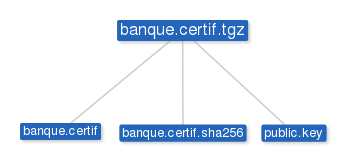
\includegraphics[scale=0.75]{banque_certif.jpg}

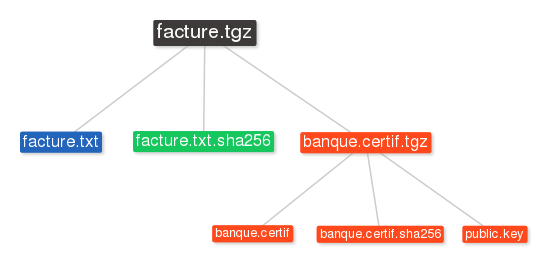
\includegraphics[scale=0.75]{facture_archi.jpg}

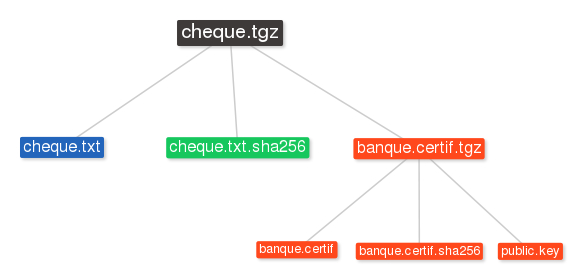
\includegraphics[scale=0.75]{cheque_archi.jpg}
\end{document}
